% Appendix B

\chapter{Appendix B: Implemented Software} % Main appendix title

\label{AppendixB} % For referencing this appendix elsewhere, use \ref{AppendixA}

The software implemented for the research is documented in the class diagram in figure \ref{fig:appB_software}.

\begin{figure}[H]
  \centering
  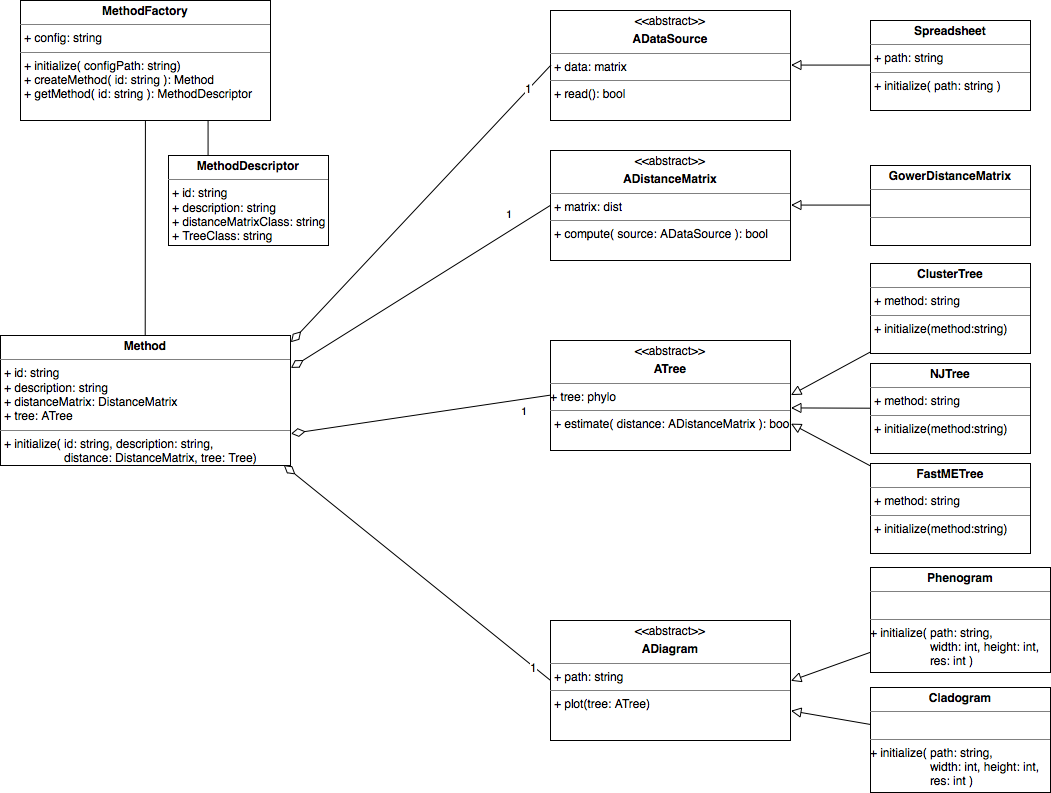
\includegraphics[width=\textwidth]{appB_software.png}
  \caption{Class diagram of the analysis software implemented for this research.}
  \label{fig:appB_software}
\end{figure}

\begin{itemize}
  \item{The \textbf{MethodFactory} takes a \textbf{MethodDescriptor} and creates a \textbf{Method} object. Method
descriptions are read from an XML configuration file. The method object aggregates a data
source, a distance matrix, a tree and a diagram objects.}
  \item{Objects extending \textbf{ADataSource} can read data exported from the database. \textbf{Spreadsheet} reads tabular data in "comma separated values" format.}
  \item{Objects extending \textbf{ADistanceMatrix} compute distances between branches.
\textbf{GowerDistanceMatrix} implements the techniques discussed in 3.1.2}
  \item{Objects extending \textbf{ATree} estimate phylogenies based on distance matrices. \textbf{ClusterTree}, \textbf{NJTree} and \textbf{FastMETree} implement the techniques discussed in 3.1.3.}
  \item{Objects extending \textbf{ADiagram} plot trees (“dendrograms”). \textbf{Phenogram} and \textbf{Cladogram} implement visualizations of taxonomic and cladistic relationships respectively.}
\end{itemize}